%
% File naaclhlt2015.tex
%
\documentclass[11pt,letterpaper]{article}
\usepackage{naaclhlt2015}
\usepackage{times}
\usepackage{latexsym}
\setlength\titlebox{6.5cm}    % Expanding the titlebox
\usepackage{amsmath}
\usepackage{multirow}
\usepackage{url}
\usepackage{graphicx}
\usepackage{hhline}
%\usepackage{natbib}
\usepackage{algorithm}
\usepackage[noend]{algpseudocode}
\usepackage{comment}
\makeatletter
\def\BState{\State\hskip-\ALG@thistlm}
\makeatother
 %\usepackage{algolyx}
%\setotherlanguage{urdu}
%\newfontfamily\urdufont[Script=Arabic,Language=Urdu,Scale=1.5]{Amiri}
%\usepackage{footnotebackref}[2012/07/01]



\DeclareMathOperator*{\argmax}{arg\,max}
\setlength\titlebox{6.5cm}    % Expanding the titlebox
%Quality Control vs. Cost Optimization in Crowdsourcing Translation%
\title{Cost Optimization for Crowdsourcing Translation}

%\author{First Author \\
%  Affiliation / Address line 1 \\
%  Affiliation / Address line 2 \\
%  Affiliation / Address line 3 \\
%  {\tt email@domain} \\\And
%  Second Author \\
%  Affiliation / Address line 1 \\
%  Affiliation / Address line 2 \\
%  Affiliation / Address line 3 \\
%  {\tt email@domain} \\}
\author{Mingkun Gao, Wei Xu \and Chris Callison-Burch\\
  Computer and Information Science Department\\
  University of Pennsylvania, Philadelphia, PA, USA\ \\
  {\tt \{gmingkun, xwe, ccb\}@seas.upenn.edu}
}
\date{}

\begin{document}
\maketitle
\begin{abstract}
Crowdsourcing makes it possible to create translations at much lower cost than hiring professional translators. However, it is still expensive to obtain millions of translations needed to train high performance statistical machine translation systems. We proposed two mechanisms to reduce the cost of crowdsourcing while maintaining high translation quality.
First, we develop a translation reducing method. We train a linear model to evaluate the translation quality on a sentence-by-sentence basis, and fit a threshold between acceptable and unacceptable translations. Unlike past work, which always paid for a fixed number of translations of each source sentence and then chose the best from them, we can stop earlier and pay less when we receive a translation that is good enough. Second, we introduce a translator reducing method by quickly identifying bad translators after they have translated only a few sentences. This also allows us to rank translators, so that we re-hire only good translators to reduce cost.   


%and so that we can select the best translations from among good candidates. 
%Additionally, we show that costs associated with gold standard calibration data created by professional translators can be reduced by using single reference instead of multiple references. 
%Besides, we reduce the cost for professional translations by reducing the number of references to calibrate each non-professional translation. 
 \end{abstract}

\section{Introduction}

Crowdsourcing is a promising new mechanism for collecting large volumes of annotated data at low cost.  %Platforms like Amazon Mechanical Turk (MTurk) provide researchers with access to large groups of people, who can complete `human intelligence tasks' that are beyond the scope of current artificial intelligence. 
%Since statistical natural language processing benefits from increased amounts of labeled training data, 
Many NLP researchers have started creating speech and language data through crowdsourcing (for example,  \newcite{snow2008}, \newcite{callison-burch-dredze2010} and others).  One NLP application that has been the focus of crowdsourced data collection is statistical machine translation (SMT) which requires large bilingual sentence-aligned parallel corpora to train translation models.  Crowdsourcing's low cost has made it possible to hire people to create sufficient volumes of translation in order to train SMT systems (for example,  \newcite{ambati2010can}, \newcite{zbib2012machine},  \newcite{post2012constructing},  \newcite{zbib2013systematic}).

However, crowdsourcing is not perfect, and one of its most pressing challenges is how to ensure the quality of the data that is created by it.  Unlike in more traditional employment scenarios, where annotators are pre-vetted and their skills are clear, in crowdsourcing very little is known about the annotators.  They are not professional translators, and there are no built-in mechanisms for testing their language skills.  They complete tasks without any oversight. Thus, translations produced via crowdousrcing may be low quality.
Previous work has addressed this problem, showing that non-professional translators hired on Amazon Mechanical Turk (MTurk) can achieve professional-level quality, by soliciting multiple translations of each source sentence and then choosing the best translation \cite{zaidan-callisonburch:2011:ACL-HLT2011a}.

In this paper we focus on a different aspect of crowdsourcing from \newcite{zaidan-callisonburch:2011:ACL-HLT2011a}.  We attempt to achieve the same high quality while {\bf minimizing the associated costs}.  
%We reduce the costs associated with non-professional translations. 
We propose two complementary methods:
(1) We reduce the number of translations that we solicit for each source sentence. Instead of soliciting a fixed number of translations for each foreign sentence, we stop soliciting translations after we get an acceptable one.  We do so by building models to distinguish between acceptable translations and unacceptable ones. (2) We reduce the number of workers we hire, and retain only high quality translators by quickly identifying and filtering out workers who produce low quality translations. Our work stands in contrast with  \newcite{zaidan-callisonburch:2011:ACL-HLT2011a} who always solicited and paid for a fixed number of translations for each source sentence, and who had no model of annotator quality. 
 
 In this paper we demonstrate that:
 \begin{itemize}
 \setlength\itemsep{0em}
 \item Our model can predict whether a given translation is acceptable with high accuracy, substantially reducing the number of redundant translations needed for every source segment.
\item Translators can be ranked well even when observing only small amounts of data. Compared with a gold standard ranking, we achieve a correlation of 0.94 after seeing the translations of only 20 sentences from each worker. Therefore, bad workers can be filtered out quickly. 
 %\item The translator ranking can also be obtained by using a linear regression model with a variety of features at a high correlation of 0.95 against the gold standard. 
 \item We can achieve a similar BLEU score as \newcite{zaidan-callisonburch:2011:ACL-HLT2011a} at half the cost using our cost optimizing methods.
 % and at 60\% of the non-professional translations' cost using model selection method.  
 \end{itemize} 
 
\section{Problem Setup}

We start with a corpus of source sentences to be translated, and we may solicit one or more translation for every sentence in the corpus.  Our targeted task is to assemble a single high quality translation for each source sentence while minimizing the associated cost. This process can be repeated to obtain multiple high quality translations.

We study the data collected by \newcite{zaidan-callisonburch:2011:ACL-HLT2011a} through Amazon's Mechanical Turk. 
They hired Turkers to translate 1792 Urdu sentences 
from the  2009 NIST Urdu-English Open Machine Translation Evaluation set\footnote{LDC Catalog number LDC2010T23}. A total of 52 Turkers contributed translations. Turkers also filled out a survey about their language skills and their countries of origin. Each Urdu sentence was translated by 4 non-professional translators (the Turkers) and 4 professional translators hired by the LDC. The cost of non-professional translation is  \$0.10 per sentence and we estimate the cost of professional translation to be approximately \$0.30 per word (or \$6 per sentence, with 20 words on average). 

Following \newcite{zaidan-callisonburch:2011:ACL-HLT2011a}, we use BLEU \cite{papineni2002bleu} to gauge the quality of human translations.  We can compute the expected quality of professional translation by comparing each of the professional translators against the other 3.  This results in an average BLEU score of  42.38.  By comparison, the Turker translations score only 28.13 on average. Zaidan and Callison-Burch trained a MERT \cite{och2003minimum,Zaidan09zmert} model to select one non-professional translation out of the four and pushed the quality of crowdsourcing translation to 38.99, closer to the expected quality of professional translation. They used a small amount of professional translations (10\%) as calibration data to estimate the goodness of the non-professional translation. The component costs of their approach are the 4 non-professional translations for each source sentence, and the professional translations for the calibration data.

Although Zaidan and Callison-Burch demonstrated that non-professional translation was significantly cheaper than professionals, we are interested in further reducing the costs.  Cost reduction plays an important role if we want to assemble a large enough parallel corpus (on the order of millions of sentence translations) to train a statistical machine translation system. 
% \cite{ambati2010can,post2012constructing,zbib2012machine,zbib2013systematic}
Here, we introduce several methods for reducing the number of non-professional translations  while still maintaining high quality. 
\section{Estimating Translation Quality}
We use a linear regression model\footnote{We used WEKA package: \url{http://www.cs.waikato.ac.nz/ml/weka/}} to predict a quality score ($ score(t) \in R$) for an input translation $t$.
%\begin{align*}
\[ score(t) = \vec{w}  \cdot \vec f(t) \]
  %\end{align*}
  where $\vec{w}$ is the associated weight vector and $\vec f(t)$ is the feature vector of the translation $t$. 

We replicate the feature set used by \newcite{zaidan-callisonburch:2011:ACL-HLT2011a} in their MERT model:

\begin{itemize}
\setlength\itemsep{0em}
\item  Sentence-level features: 9 features based on language model, sentence length and edit distance to other translations. 
\item Worker-level features: 15 features based on worker's language ability, location and average sentence-level scores.
\item Ranking features: 3 features based on the judgments of monolingual English speakers' ranking the translations from best to worst.
\item Calibration features: 1 feature based on the average BLEU score of a worker's translations provided is computed against professional references.
%\item Bilingual features: 1 feature based on the word alignment probabilities according. 
\end{itemize}


We additionally introduce a new bilingual feature based on IBM Model 1. We align words between each candidate translation and its corresponding source sentence. The bilingual feature for a translation is the average of its alignment probabilities. In Figure \ref{biexample1}, we show how the bilingual feature allows us to distinguish between a valid translation (top) and an invalid/spammy translation (bottom).

\begin{figure}
  \centering
  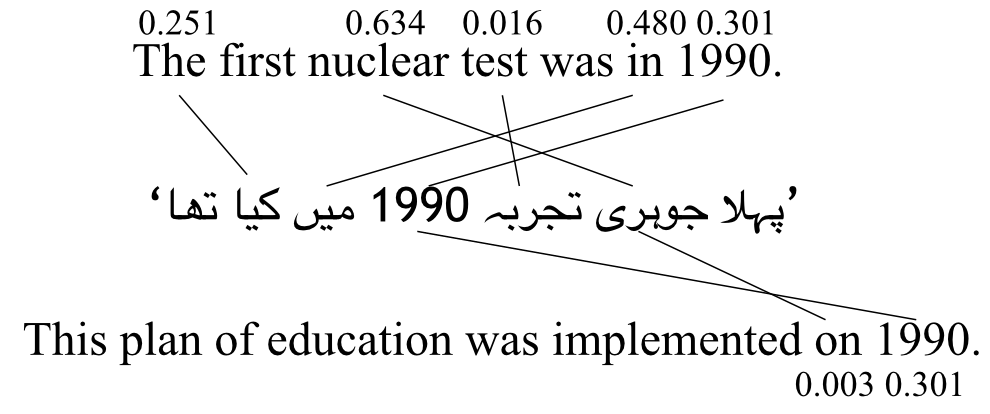
\includegraphics[width=\linewidth]{bilingualexample/example.png}
  \caption{Example bilingual features for two crowdsourced translations of an Urdu sentence. The numbers are alignment probabilities for each aligned word. The bilingual feature is the average of these probabilities, thus 0.240 for the good translation and 0.043 for the bad translation. Some words are not aligned if potential word pairs don't exist in bilingual training corpus.
}
    \label{biexample1}
\end{figure}

%\newcite{zaidan-callisonburch:2011:ACL-HLT2011a} used all 4 professional translations in computing the calibration features and training labels. We will show in the experiments that using \textbf{only one} professional translation as reference is as sufficient. 


\begin{algorithm}[h!]
\textbf{Input}: $\delta$, the allowable deviation from the expected upper bound on BLEU score (using all redundant translations); $\alpha$, the upper bound BLEU score; a training set $S = \{\vec f^{s}_{i,j},y^{s}_{i,j})_{i=1..n}^{j=1..m}\}$ and a validation set $V = \{(\vec f^{v}_{i,j},y^{v}_{i,j})_{i=1..n}^{j=1..m}\}$ where $\vec f_{i,j}$ is the feature vector for $t_{i,j}$ which is the $jth$ translation of the source sentence $s_{i}$ and $y_{i,j}$ is the label for $\vec f_{i,j}$.\\
\textbf{Output}: $\theta$, the threshold between acceptable and unacceptable translations; $\vec{w}$, a linear regression model parameter. 
\begin{algorithmic}[1]
\State \textbf{initialize} $\theta \leftarrow 0$,$\vec{w}\leftarrow \emptyset$ 
\State $\vec{w'}\leftarrow$ train a linear regression model on $S$
\State $maxbleu \leftarrow$ select best translations for each $s_i \in S$ based on the model parameter $\vec{w'}$ and record the highest model predicted BLEU score
\While {$\theta \neq maxbleu $} 
\For {$i \leftarrow 1$ to $n$}
\For {$j \leftarrow 1$ to $m$}
\If {$\vec{w'}\cdot \vec f^v_{i,j} > \theta \wedge j < m $}
             select $t^{v}_{i,j}$ for $s_i$ and \textbf{break}
\EndIf
\If {$ j == m $} select $t^{v}_{i,m}$ for $s_i$
\EndIf
\EndFor
\EndFor
\State $q \leftarrow$ calculate translation quality for V
\If {$q > \delta \cdot \alpha$} \textbf{break}
\Else \text{  } $\theta = \theta + stepsize$
\EndIf
\EndWhile
\State $\vec {w} \leftarrow$ train a linear regression model on $S \cup V$
\State \textbf{Return}: $\theta$ and model parameter $\vec{w}$
%\EndProcedure
\end{algorithmic}
\caption{Model Training Algorithm}\label{modelselection}
\end{algorithm}



\section{Reducing the Number of Translations}
The first mechanism that we introduce to optimize cost is to solicit less translations.  The strategy is to recognize when we have got a good translation of a source sentence and to immediately stop purchasing additional  translations of that sentence.  The crux of this method is to decide whether a translation  is `good enough,' in which case we do not gain any benefit from  paying for another redundant translation.  

Our translation reduction method allows us to set an empirical definition of `good enough'.  
We define an Oracle upper bound $\alpha$ to be the estimated BLEU score using the full set of non-professional translations.
We introduce a parameter $\delta$ to set the allowable degradation in translation quality. We train a model to search for a threshold $\theta$ between acceptable and unacceptable translations for a specific value of $\delta$. For instance, we may fix $\delta$ at 95\%, meaning that the resulted BLEU score should not drop below 95\% of the $\alpha$ after reducing the number of translations.   

For a new translation, our model scores it, and if its score is higher than $\theta$, then we do not solicit another translation. Otherwise, we continue to solicit translations.  Algorithm \ref{modelselection} details the process of model training and searching for $\theta$. 


 \begin{table}
 \center
\begin{tabular}{c|c|c}
\hline
$\delta$(\%) & BLEU Score & \# Trans. \\ \hhline{===}
90    & 36.26      & 1.63            \\
91    & 36.66      & 1.69             \\
92    & 36.93      & 1.78             \\
93    & 37.23      & 1.85             \\
94    & 37.48      & 1.93             \\
95    & 38.05      & 2.21             \\
96    & 38.16      & 2.30             \\
97    & 38.48      & 2.47             \\
98    & 38.67      & 2.59             \\
99    & 38.95      & 2.78             \\
100   & 39.54      & 3.18             \\ \hline
\end{tabular}
\caption{The relation among the $\delta$ (the allowable deviation from the expected upper bound on BLEU score), the BLEU score for translations selected by models from partial sets and the averaged size of translation candidates set for each source sentence (\textit{\# Trans}).  }
    \label{orderanother}
\end{table}


\subsection{Experiments}
 We divide data into a training set (10\%), a validation set (10\%) and a test set (80\%). Each source sentence has four translations in total. We use the validation set to search for $\theta$.  The Oracle upper bound on BLEU is set to be 40.13 empirically. 
We then vary the value of $\delta$ from 90\% to 100\%, and sweep values of $\theta$ by incrementing it in step sizes of 0.01.
We report results based on a five-fold cross validation, rotating the training, validation and test sets.

\subsubsection{Baseline and upper bound} 
The baseline selection method of randomly picking one translation for each source sentence achieves a BLEU score of 29.56. To establish an upper bound on translation quality, we perform an oracle experiment to select best translation for each source segment from full sets of candidates.  It reaches a BLEU score of 40.13.

\subsubsection{Translation reducing method} 

Table \ref{orderanother} shows the results for translation reducing method.  The $\delta$ variable correctly predicts the deviation in BLEU score when compared to using the full set of translations.   If we set $\delta$ $<$ 0.95 then we lose 2 BLEU points, but we cut the cost of translations in half, since we pay for only two translations of each source segment on average.


\begin{figure}
  \centering
  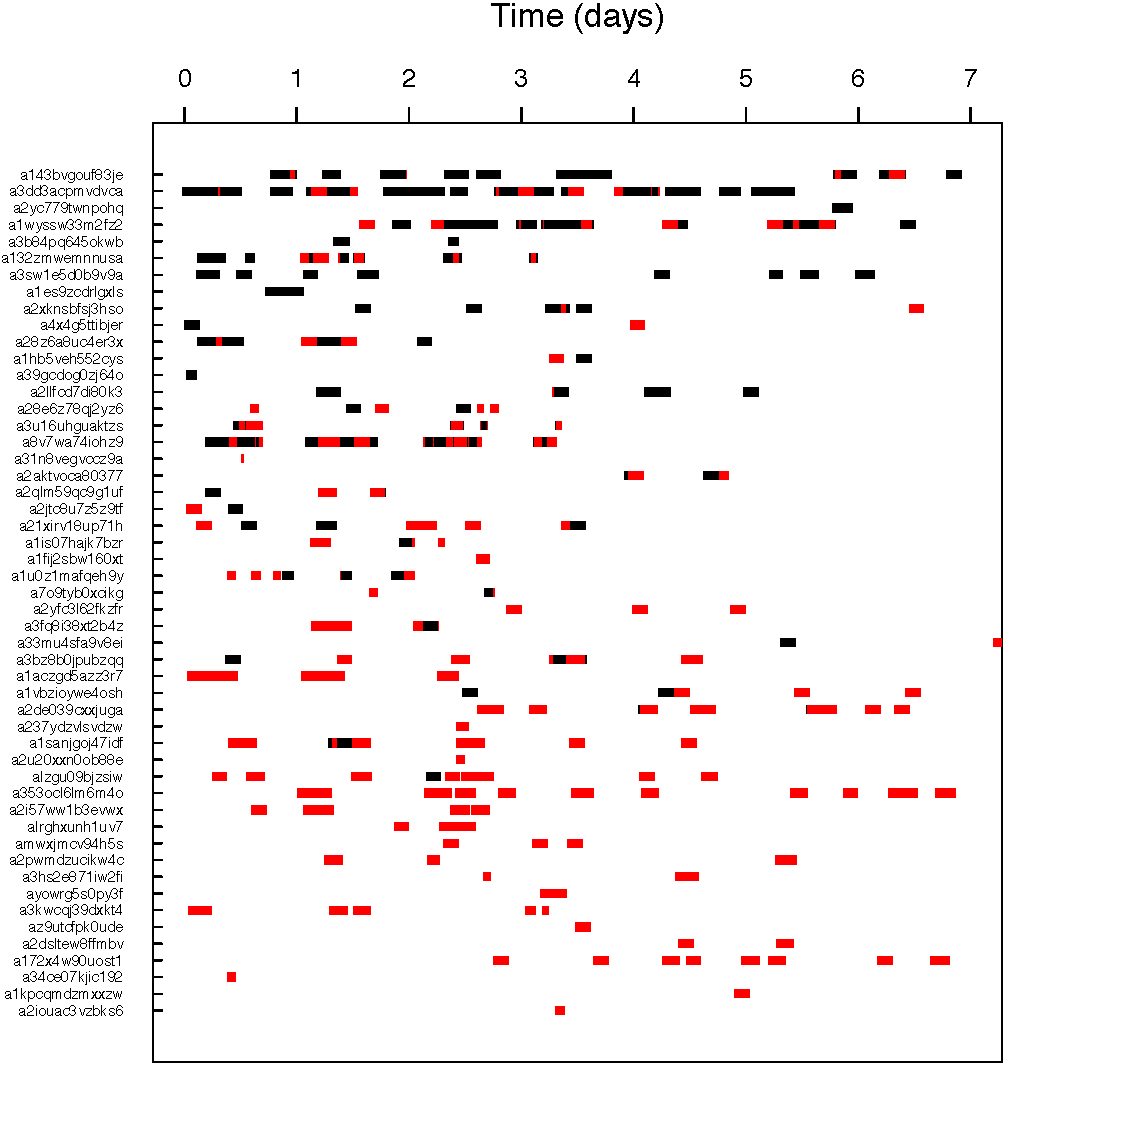
\includegraphics[width=\linewidth]{WorkerPerf/wp.pdf}
  \caption{A time-series plot of all of the translations produced by Turkers (identified by their WorkerID serial number). Turkers are sorted with the best translator at the top of the y-axis. Each tick represent a single translation and black color means better than average quality.
}
    \label{fworkerperf}
\end{figure}


\section{Choosing Better Translators}

The second mechanism that we use to optimize cost is to reduce the number of non-professional translators that we hire.  Our goal is to quickly identify whether Turkers are good or bad translators, so that we can continue to hire only the good translators and stop hiring the bad translators after they are identified as such. 
%
Before presenting our method, we first demonstrate that Turkers produce consistent quality translations over time.


\subsection{Turkers' behavior in translating sentences}

Do Turkers produce good (or bad) translations consistently or not? Are some Turkers  consistent and others not? We used the professional translations as a gold-standard to analyze the individual Turkers, and we found that most Turkers' performance stayed surprisingly consistent over time. 

Figure \ref{fworkerperf} illustrates the consistency of workers' quality by plotting quality of their individual translations on a timeline. The translation quality is computed based on the BLEU against professional translations. Each tick represent a single translation and depicts the BLEU score using two colors. The tick is black if its BLEU score is higher than the median and it is red otherwise. Good translators tend to produce consistently good translations and bad translators rarely produce good translations.





 \begin{figure*}[!ht]
\centering
\begin{minipage}[t]{.475\textwidth}
 \centering
  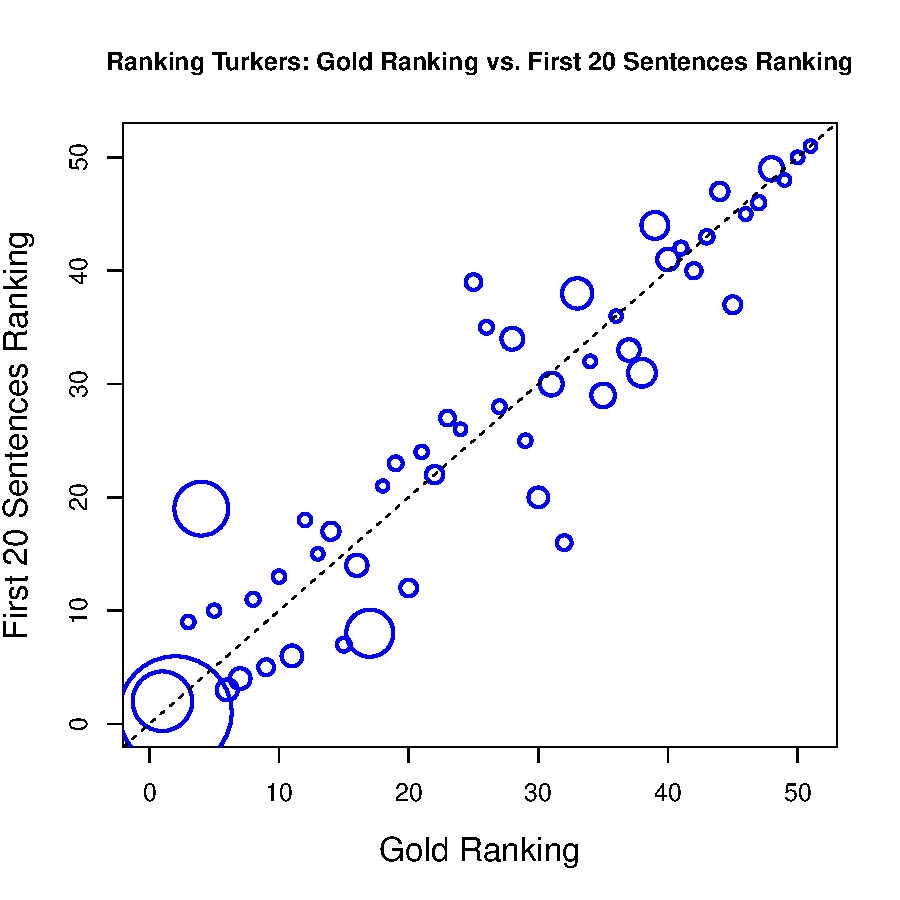
\includegraphics[width=2.8in]{AllFeatureWithCali/2hitranking.pdf}
   \caption{Correlation between gold standard ranking and ranking computed using the first 20 sentences as calibration. Each bubble represents a worker. The radius of each bubble shows the relative volume of translations completed by the worker. 
The  weighted correlation is 0.94.  }
\label{first2hitrank}
\end{minipage}
\hfill
\begin{minipage}[t]{.475\textwidth}
  \centering
  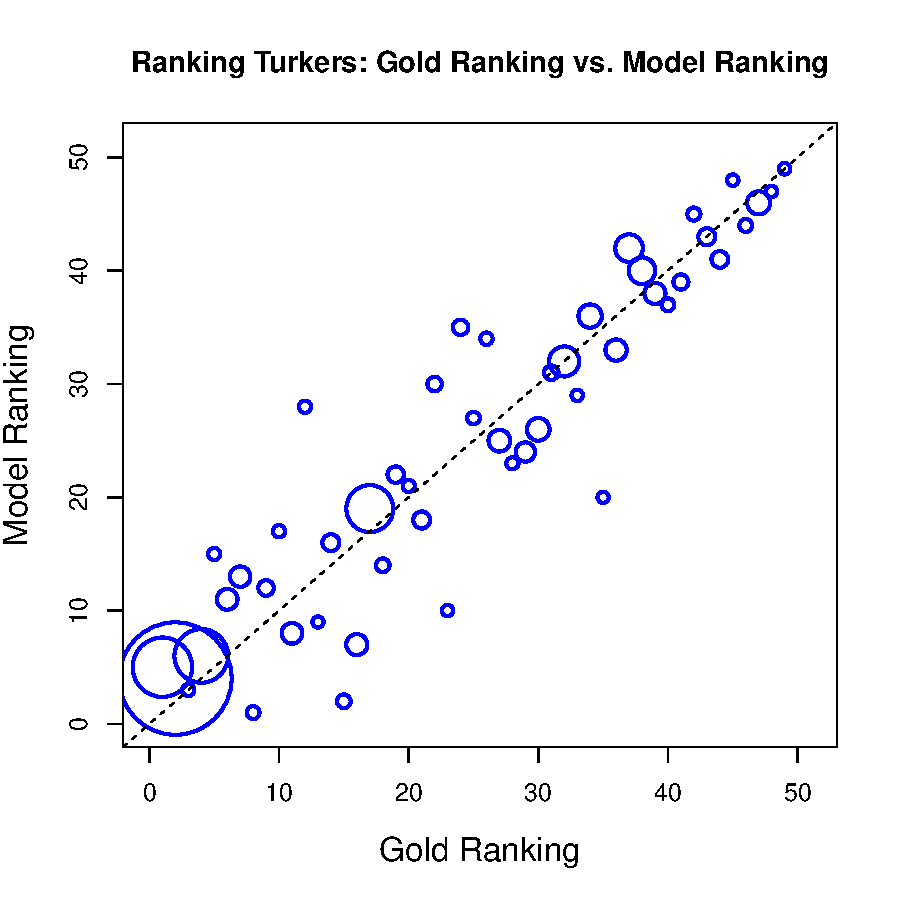
\includegraphics[width=2.8in]{AllFeatureWithCali/allfeaturelinear.pdf}
  \centering
     \caption{Correlation between gold standard ranking and our model's ranking. 
The corresponding weighted correlation is 0.95.}
  \label{modelrank}
\end{minipage}
\end{figure*}


\begin{comment}
\begin{figure}
  \centering
  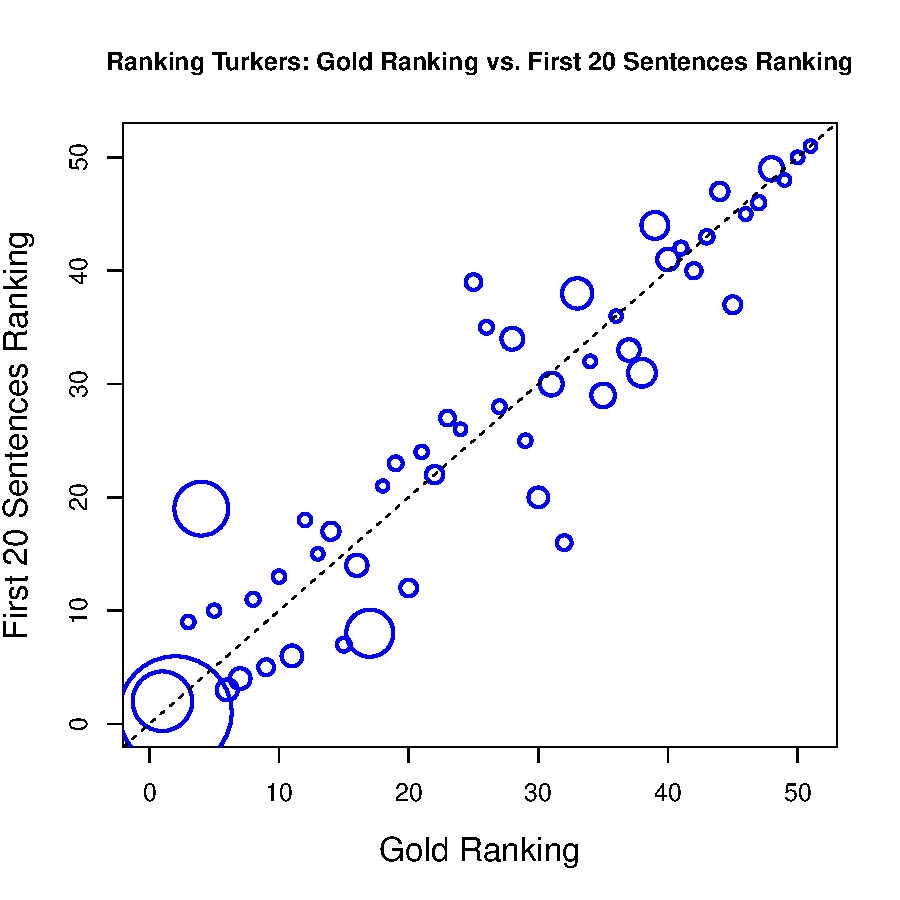
\includegraphics[width=\linewidth]{AllFeatureWithCali/2hitranking.pdf}
  \caption{Correlation between gold standard ranking and ranking computed using the first 20 sentences as calibration. Each bubble represents a worker. The radius of each bubble shows the relative volume of translations completed by the worker. 
The  weighted correlation is 0.94.  }
    \label{first2hitrank}
\end{figure}
%
\begin{figure}
  \centering
  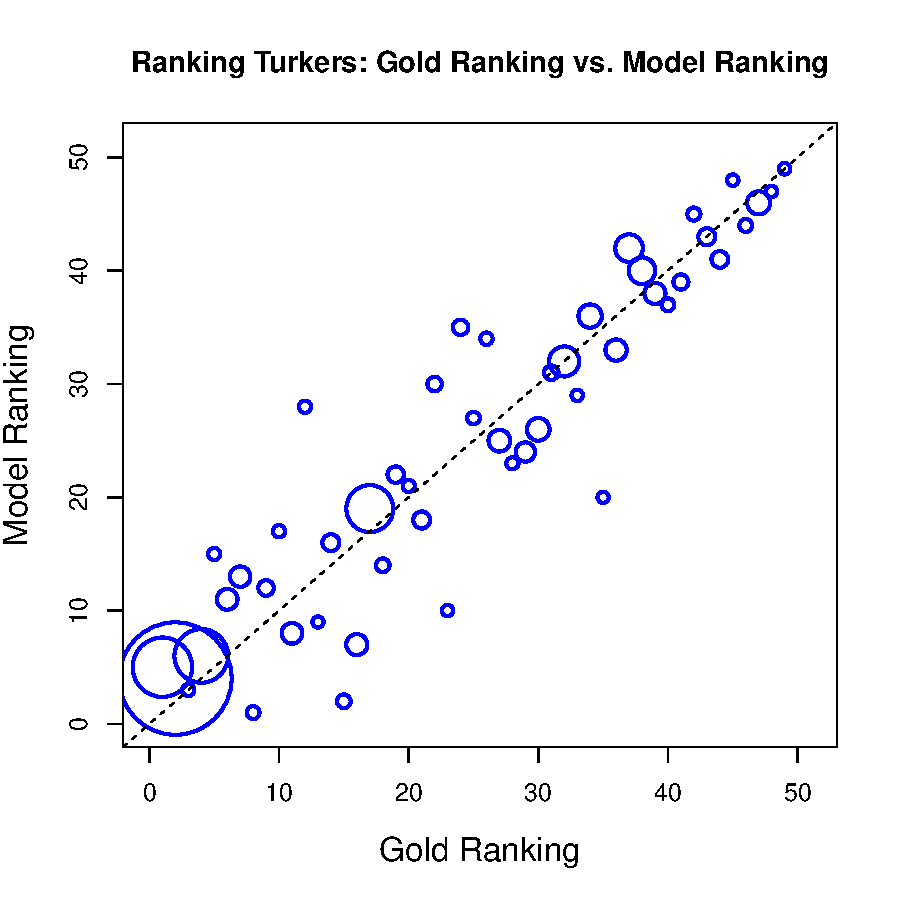
\includegraphics[width=\linewidth]{AllFeatureWithCali/allfeaturelinear.pdf}
  \caption{Correlation between gold standard ranking and our model's ranking. 
The corresponding weighted correlation is 0.95.}
    \label{modelrank}
\end{figure}
\end{comment}


\subsection{Evaluating Rankings}
We use weighted Pearson correlation \cite{pozzi2012exponential} to evaluate our ranking of workers against gold standard ranking. Since workers translated different number of sentences, it is more important to rank the workers who translated more sentences correctly. Taking the importance of workers into consideration, we set a weight to each worker using the number of translations he or she submitted when calculating the correlation.
Given two lists of worker scores \textit{x} and \textit{y} and the weight vector \textit{w}, the weighted Pearson correlation $\rho$ can be calculated as:
\begin{equation}
\rho(x,y;w) = \frac{cov(x,y;w)}{\sqrt{cov(x,x;w)cov(y,y;w)}}
\end{equation}
where $cov$ is weighted covariance:
\begin{equation}
cov(x,y;w)  = \frac{\sum_i w_i (x_i - m(x;w))(y_i - m(y;w))}{\sum_i w_i}
\end{equation}
and $m$ is weighted mean:
\begin{equation} 
m(x;w)  =  \frac{\sum_{i} w_i x_i}{\sum_i w_i} 
\end{equation}

\subsection{Automatically Ranking Translators}

We introduce two approaches to rank workers using a small portion of the work that they submitted.  The strategy is to filter out bad workers, and to select the best translation from translations provided by the remaining workers. We propose two different ranking methods:


%We present translator reducing methods to compute ranks of workers from a small portion of work they submitted. We filter out bad workers and select the best translation from translations provided by  surviving workers.
%The consistency of workers' performance and the comparability of translation qualities between selecting translations by workers' ranks and selecting translations by models  are two preconditions guarantee this mechanism works.


%They are both very 'cheap' since we only use a small portion of professional translations and avoid hiring bad workers after we get workers' ranking.  
% and evaluate the translation quality by calculating the BLEU score against references.

\paragraph{Ranking workers using their first $k$ translations}
We rank the Turkers using their first few translations by comparing their translations against the professional translations of those sentences. Ranking workers on gold standard data would allow us to discard bad workers. This is similar to the idea of a qualification test in MTurk. 

\paragraph{Ranking workers using a model}
In addition to ranking workers by comparing them against a gold standard, we also attempt to automatically predict their ranks with a model. 
We use the linear regression model to score each translation and rank workers by their model predicted performance.  
%For each source sentence $s_i$, we have a translation set $T = \{ t_{i,1}, t_{i,2},t_{i,3}, t_{i,4}\}$. 
 The model predicted performance of the worker $w$ is:
\begin{equation}
performance(w) = \frac{\sum_{t \in T_{w}} score (t)}{|T_{w}|}
\end{equation}
where $T_{w} $ is the set of translations completed by the worker $w$ and  $score(t)$ is the model predicted score for translation $t$. 
 

\subsection{Experiments}

After we rank workers, we keep top-ranked workers and select the best translation only from their translations. For both ranking approaches, we vary the number of good workers that we retain. 

We report both rankings' correlation with the gold standard ranking. Since the top worker threshold is varied and since we change the value of k in first k sentence ranking, we have a different test set in different settings. Each test set excludes any items which were used to rank the workers, or which did not have any translations from the top workers according to our rankings. 
%In addition to evaluating the correlation of our different ways of ranking translators, 
We also compute the translation quality when selecting the translation provided by the worker with best rank.



\subsubsection{Gold standard and Baseline}
We evaluate ranking quality using the weighted Pearson correlation ($\rho$) compared with the gold standard ranking of workers. 
To establish the gold standard ranking, we score each Turker based on the BLEU score comparing all of his or her translations to the corresponding professional references.

We use the ranking by the MERT model developed by \newcite{zaidan-callisonburch:2011:ACL-HLT2011a} as baseline. It achieves a correlation of 0.73 against the gold standard ranking. 


% in gold standard ranking, and the BLEU score achieved is denoted as $B_{gold}$.
%Besides, we set the random selection method as the naive baseline method which randomly select a translation from all candidates for each source sentence. 


\subsubsection{Ranking workers using their first $k$ translations}
 Without using any model, we rank workers using their first k translations. We select best translation of each source sentence from the top ranked worker who translated that sentence. To evaluate this method, we calculate the weighted correlation for our rankings against gold ranking. 
 %we created several test sets.  Each test set excluded any item that was used to rank the workers, or which did not have any translations from the top 25\% of workers according to our predicted rankings.  We therefore have \emph{different test sets} for each value of k.  This makes the results slightly more difficult to analyze than in normal experiments, although the trends are still clear.
%Formally, we define the test set for first k sentences as $T_k$ and for each source sentence $s \in T_k$:
%\begin{align*}
%  \{ s \mid (C(s) \cap S_k = \emptyset)   \wedge (C(s) \cap S_w \neq \emptyset)    \}
%\end{align*}
%where $C(s)$ is the translating candidates set of the source sentence $s$, $S_k$ is the translation set consists of each worker's first k translations and $S_w$ is the translation set consists of translations provided by selected workers (some top ranking workers). 

Table \ref{spearmansen} shows the results of Pearson correlations for different value of $k$. As $k$ increases, our rankings fit to the gold ranking better. Consequently, we can decide whether to continue to hire a worker in a very short time after analyzing the first k sentences ($k\le20$) provided by each worker. Figure \ref{first2hitrank} shows the correlation of gold ranking and first 20 sentences ranking. 

%Table \ref{first20toprank} shows similar results as Table \ref{modeltoprank}. We can achieve a translation quality close to that of gold ranking selection with only soliciting half of non-professional translations if we keep hiring top 25\% workers after seeing 20 translations submitted from each of them.
%\begin{table}
%\center
%\begin{tabular}{c|ccccc}
%\hline
%Top(\%) &$B_{r}$& $B_{t}$ & $B_{gold}$ & $\Delta$ & \# of Trans\\\hhline{======}
%25      &28.76& 36.97   & 37.10      & 0.13   & 2.03         \\
%50      &29.27& 36.90   & 37.15      & 0.25   & 2.60         \\
%75      &28.89& 36.77   & 37.06      & 0.29   & 3.47         \\
%100     &27.51&   36.77 & 37.06      & 0.29   & 4.00         \\ \hline
%\end{tabular}
%\caption{\label{first20toprank}The comparison between translation quality of selecting translations based on first 20 sentences ranking ($B_{t}$) and gold ranking ($B_{gold}$) when we keep hiring different percentages of top workers. $\Delta$ is the different between $B_{gold}$ and $B_t$. \# of Trans is the average number of non-professional translations needed for each source sentence. $B_r$ is the BLEU score for random selection.
%}
%\end{table} 



\subsubsection{Ranking workers using a model}
We train a linear regression model on 10\% of the data to rank workers.  We use the model to select the best translation in one of two ways:
\begin{itemize}
\setlength\itemsep{0em}
\item By using the model's prediction of workers' rank, and selecting the translation from the best worker.  
\item By using the model's score for each translation and selecting the highest scoring translation of each source sentence. 
\end{itemize}

Table \ref{lrresult} shows that the model trained on all features achieves a very high correlation with the gold standard ranking (Pearson's $\rho$ = 0.95), and a  BLEU score of 39.80.



Figure \ref{modelrank} presents a visualization of the gold ranking and model ranking. The workers who produce the largest number of translations (large bubbles in the figure) are ranked extremely well.


\subsection{Filtering out bad workers}

Ranking translators would allow us to reduce costs, by only re-hiring top workers.
 Table \ref{modeltoprank} shows what happens when we vary the top percentage of workers we retain.  In general, the model does a good job of picking the best translations from the remaining good translators.  Comparing against knowing the gold ranking, the model loses only 0.55 BLEU when we filter out 75\% of the workers.  In this case we only need to solicit two translations for each source sentence on average.


\begin{table}
\begin{center}
\begin{tabular}{cc|c}
\hline
\multicolumn{2}{c|}{\begin{tabular}[c]{@{}c@{}}Proportion of \\ Calibration Data\end{tabular}} & \multirow{2}{*}{\begin{tabular}[c]{@{}c@{}}$\rho$\end{tabular}}\\ \cline{1-2}
% & \multirow{2}{*}{\begin{tabular}[c]{@{}c@{}}$\rho^{*}$\end{tabular}} \\ \cline{1-2}
First k sentences                                 & Percentage                                 &                                                                                                                                          \\ \hhline{===}
1                                                 & 0.7\%                                      & 0.21 \\
2                                                 & 1.3\%                                      & 0.38 \\
3                                                 & 2.0\%                                      & 0.41 \\
4                                                 & 2.7\%                                      &  0.56\\
5                                                 & 3.3\%                                      & 0.70                                                                                                                            \\
%6                                                 & 4.0\%                                      & 0.75                                                                                                                                 \\
%7                                                 & 4.7\%                                      & 0.76                                                                                                                                    \\
%8                                                 & 5.3\%                                      & 0.73                                                                                                                                    \\
%9                                                 & 6.0\%                                      & 0.78                                                                                                                                  \\
10                                                & 6.6\%                                      & 0.81                                                                                                                                    \\
20                                                & 13.3\%                                     & 0.94 \\
30                                                & 19.9\%                                     & 0.96 \\
40                                                & 26.6\%                                     & 0.98 \\
50                                                & 33.2\%                                     & 0.98                                                                                                                                   \\ 
60                                                & 39.8\%                                     & 0.98 \\ \hline
\end{tabular}
\end{center}
\caption{\label{spearmansen} Pearson Correlations for calibration data in different proportion. 
%* indicates that the calibration is computed against \textbf{only one} reference while + indicates that the calibration is computed against 4 references.
}
\end{table}

\begin{table}[htbp]
 \center
\begin{tabular}{c|c|cc}
\hline
 & & \multicolumn{2}{c}{BLEU}\\
Feature Set             & $\rho$  & rank & score    \\ \hhline{====}
(S)entence features     & 0.80 & 36.66 &37.84 \\
(W)orker features       & 0.78 & 36.92 &36.92 \\
(R)anking features      & 0.81 & 36.94 &35.69\\
Calibration features  & 0.93 & 38.27 &38.27\\
%Calibration features* & \textbf{0.68} & \textbf{37.22} \\
S+W+R features          & 0.86 & 37.39 & 38.69\\
S+W+R+Bilingual features        & 0.88 & 37.59 &39.23 \\
All features            & \textbf{0.95} & \textbf{38.37} & \textbf{39.80}\\ \hhline{====}
Baseline (MERT) &0.73&-&38.99\\ \hline
%All features*            & \textbf{0.71} & \textbf{37.52} \\ \hline
\end{tabular}
\caption{\label{lrresult} Correlation ($\rho$) and translation quality for the various features used by our model.  Translation quality is computed by selecting best translations based on model-predicted workers' ranking (rank) and model-predicted translations' scores (score). Here we do not filter out bad workers when selecting the best translation.}
\end{table}



\begin{table}[htbp]
\center
\begin{tabular}{c|ccccc}
\hline
Top & \multicolumn{4}{c}{BLEU}&\\
 (\%) &random & model & gold & $\Delta$ & \# Trans\\\hhline{======}
25      &29.85& 38.53   & 39.08      & 0.55   & 1.95         \\
50      &29.80& 38.40   & 39.00      & 0.60   & 2.73         \\
75      &29.76& 38.37   & 38.98      & 0.61   & 3.48         \\
100     &29.83& 38.37   & 38.99      & 0.62   & 4.00         \\ \hline
\end{tabular}
\caption{\label{modeltoprank} A comparison of the translation quality when we retain the top translators under different rankings.  The rankings shown are random, the model's ranking (using all features from Table \ref{lrresult}) and the gold ranking.  $\Delta$ is the different between the BLEU scores for the gold ranking and the model ranking. \# Trans is the average number of translations needed for each source sentence. 
}
\end{table} 


\section{Cost Analysis}

 We have introduced several ways of significantly lowering the costs associated with crowdsourcing translations when a large amount of data are solicited (on the order of millions of samples):
\begin{itemize}
\setlength\itemsep{0em}
\item We show that after we have collected one translation of a source sentence, we can consult a model that predicts whether its quality is sufficiently high or whether we should pay to have the sentence re-translated.  The cost savings for non-professionals here comes from reducing the number of redundant translations. We can save half of the cost associated with non-professional translations to get 95\% of the translation quality using the full set of redundant translations.
\item We show that we can quickly identify bad translators, either by having them first translate a small number of sentences to be tested against professional translations, or by estimating their performance using a feature-based linear regression model. The cost savings for non-professionals here comes from not hiring bad workers. Similarly, we reduce the non-professional translation cost to the half of the original cost.

\item In both cases we need some amount of professionally translated materials  to use as a gold standard for calibration. Although the unit cost for each reference is much higher than the unit cost for each non-professional translation, the cost associated with non-professional translations can dominate the total cost since the large amount of data need to be collected. Thus, we focus on reducing cost associated with non-professional translations. 
%The cost savings for professionals come from reducing the referencing translations to calibrate each data sample. 
% The cost of these professional translations can dominate the cost of our models, so we experiment with how little we can get away with.
\end{itemize}
%In all cases, there is a trade-off between lowering our costs and producing high quality translations.  Figure \ref{fbleucost} plots the cost versus the BLEU scores for the different configurations that we experimented with.
%
%In Figure \ref{fbleucost}-(a) the increasing costs are a function of how many sentences we use to rank the translators.  Here we use no model, and simply rank the translators by their BLEU score against a small amount of gold standard data. The quality peaks at 37.9 BLEU after \$3,000.
%%the return on investment is low after spending the first \$2,000 to get a BLEU of 35.6.
%We are able to rank the translators with high accuracy and achieve a relative high BLEU score by paying for a comparatively small number of professional translations to use as calibration. From our experiments,  10-20 professionally translated sentences seems like a reasonable number. 
%
%Figure\ref{fbleucost}-(b) uses a model to determine whether to purchase another translation.  
%%Here the starting cost is high (nearly \$9,000) because the model requires a significant amount of professional translations in order to train the model and to determine the optimal threshold values for whether to solicit another translation. 
%This model allows us to significantly improve the overall translation quality to a BLEU score of nearly 40, for a final cost of \$2,700.
%
%%To emphasize the effectiveness of model selection approach, Figure \ref{fbleucost}-(c) plots the relationship between BLEU and non-professional component of the overall cost.  Past approaches to crowdsourcing translation always solicited 4 non-professional translations of every source sentence. The cost for translating our 1433 test sentences under this approach is \$573.44.  This produces the maximum BLEU score of 40.1.  Using our model to reduce the number of redundant translations, we can reduce the costs with mild degredation in translation quality.  We can cut the number of non-translations in half, and pay only \$286.72, while achieving a BLEU score of 37.6 (94\% of the maximum), or pay \$348.36,60.7\% of total non-professional translations' cost, for a BLEU of 38.5 (96\% of  the maximum).
%
%\begin{figure}[htbp]
%  \centering
%  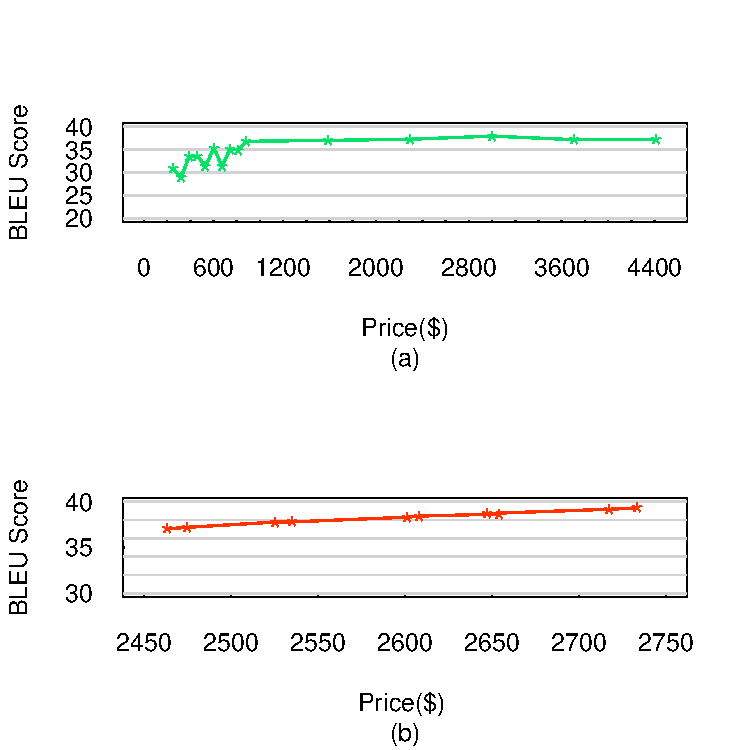
\includegraphics[width=\linewidth]{cost-bleu/pricecost.pdf}
%  \caption{The Relationship between BLEU score and costs. In Figure (a), the red line shows the relationship between BLEU score and  the total costs (professional and non-professional) for the ranking based approach. 
%  %The green line shows the corresponding translation quality for gold standard ranking selection measured in BLEU score. 
%  Figure (b) shows the relationship between BLEU score and the total costs for model-based approach. 
%  %Figure (c)  illustrates the relationship between BLEU score and non-professional costs for model based approach.
%  }
%    \label{fbleucost}
%\end{figure}
\section{Related Work}
%Crowdsoucing has been widely used in data annotation or labeling to get a large amount of data at low cost. The relationship between the budget and the quality was discussed in previous work.

\newcite{sheng2008get} focused on training a machine learning model from noisy labels.
%repeated labeling presents a way of solving the problems of uncertainty in labeling. 
We cannot always get high-quality labeled data from crowdsourcing, but we can still ensure that a model trained on the data accurate by redundantly labeling the data.
%samples with relatively low costs, to keep the model trained on noisy labeled data having a high accuracy in predicting, 
\newcite{sheng2008get} proposed a framework for repeated-labeling that resolves the uncertainty in labeling via majority voting. The experimental results show that a model's accuracy is improved even if labels in its training data are noisy and imperfect.
% and of imperfect quality.  
As long as the integrated quality (the probability of the integrated labeling being correct) is higher than 0.5, repeated labeling benefits model training. 

\newcite{passonneau2013benefits} created a Bayesian model of annotation. They applied it to the problem of word sense annotation. \newcite{passonneau2013benefits} also proposed an approach to detect and avoid spam workers. 
They measured the performance of worker by comparing worker's labels to the current majority labels and worker with bad performance can be blocked. 
%However, this approach may suffer from two shortcomings: 1) sometimes majority labels may not reflect the ground truth label; 2) they didn't figure out  how much data (HITs) is needed to evaluate a worker's performance. Although they could find the spam after the fact, it might be a post-hoc analysis, so they might have already wasted the money to pay for a spam worker who should have been detected earlier.

\newcite{lin2014re} examined the relationship between worker accuracy and budget in the context of using crowdsourcing to train a machine learning classifier.  They show that if the goal is to train a classifier on the labels, that the properties of the classifier will determine whether it is better to re-label data (resulting in higher quality labels) or get more single labeled items (of lower quality). They showed that classifiers with weak inductive bias  benefit more from relabeling, and that relabeling is more important when worker accuracy is low. %(barely higher than 0.5). 

\newcite{novotney2010cheap} showed a similar result for training an automatic speech recognition (ASR) system.  When creating training data for an ASR system, given a fixed budget. Their system's accuracy was higher when it is trained on more low quality transcription data compared to when it was trained on fewer high quality transcriptions.


\section{Conclusion}
In this paper, we propose two mechanisms to optimize cost: a translation reducing method and a translator reducing method. They have different applicable scenarios for large corpus construction.
The translation reducing method works if there exists a specific requirement that the quality control must reach a certain threshold. 
This model is most effective when reasonable amounts of pre-existing professional translations are available for setting the model's threshold. 
The translator reducing method is very simple and easy to implement. This approach is inspired by the intuition that workers' performance is consistent. The translator reducing method is suitable for crowdsourcing tasks which do not have specific requirements about the quality of the translations, 
or when only very limited amounts of gold standard data are available.

\section*{Acknowledgements}

This material is based on research sponsored by a DARPA Computer Science Study Panel phase 3 award entitled ``Crowdsourcing Translation'' (contract D12PC00368). The views and conclusions contained in this publication are those of the authors and should not be interpreted as representing official policies or endorsements by DARPA or the U.S. Government. This research was supported by the Johns Hopkins University Human Language Technology Center of Excellence and through gifts from Microsoft, Google and Facebook.

 \bibliographystyle{naaclhlt2015}
\bibliography{naaclhlt2015_new}

\end{document}